\documentclass[conference]{ieeetran}
\usepackage{authblk}
\usepackage{graphicx}
\graphicspath{ {./images/} }
%\usepackage{babel}
\usepackage{amsmath}

\author[1]{Jay Piamjariyakul}
%\author[2]{Felix Kong}
\affil[1]{Department of Electrical \& Electronic Engineering, University of Bristol}
%\affil[2]{Department of Mechanical Engineering, University of Bristol}
\title{Your Foot in the Pave: Generating Electricity with Footsteps}

\renewcommand\IEEEkeywordsname{Keywords}
\newcommand{\figref}[1]{\figurename~\ref{#1}}

\begin{document}

\maketitle
\begin{abstract}
This document examines the plausibility \& efficiency of generating power via footsteps, which could be used on pavements to generate electricity used for various purposes, depending on the user's preferences.
\end{abstract}

% \begin{IEEEkeywords}
%     Broad band networks, quality of service, WDM.
% \end{IEEEkeywords}
 
% \section{Preamble}
% The application of utilising footsteps to generate electricity adapts the mechanisms of a dynamo (which generates electricity from mechanical torque input) and that of a pressure plate (akin to those used in vintage spinning-top toys). Its applications, theoretically, could be used to alleviate lack of electricity in remote regions (given a large amount of foot-based commuting) or help local businesses collect data in regards to visitors/browsers \& determine their best course of business action.

\section{Mechanism Proposal}
The proposed mechanism to generate electricity is comprised of multiple components, and such operate in unison to provide the output voltage at the output stage.

\subsection{Components Analysis}
The mechanism itself involves a button/plate that, when pressed, would push a spiral down an entry point, compressing a spring. When such button/plate (thus, the spring) is released, the spiral is released to its initial position, in turn spinning the flywheel disc/gear that such spiral is fixed to, causing such to move in a rotational manner.

\begin{figure}[ht]
    \centering
    \caption{Diagram of proposed mechanism to generate electricity from footsteps}
    \label{fig:mechanism_side_wlabel}
    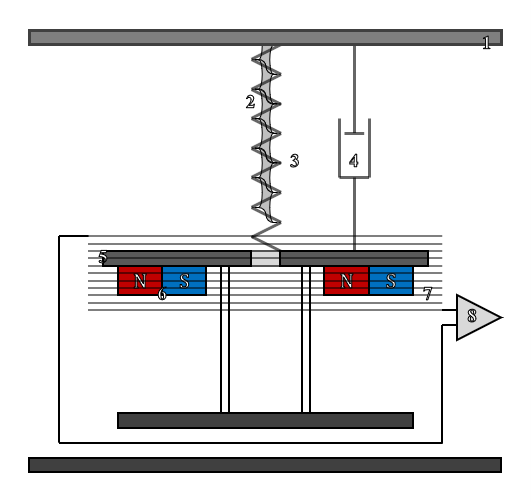
\includegraphics[width=\linewidth]{mechanism_side_wlabel.png}
\end{figure}

\begin{figure}[ht]
    \centering
    \caption{Top-down view of spiral-driven gear \& its attached magnets}
    \label{fig:mechanism_winding_top}
    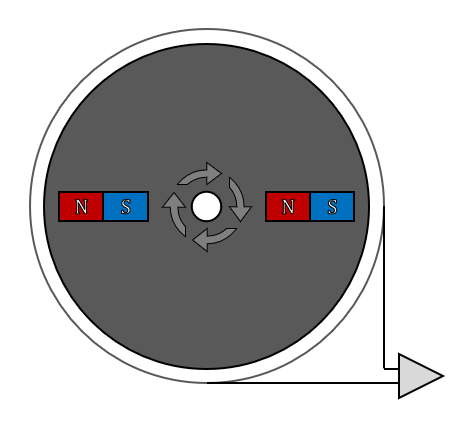
\includegraphics[width=0.6\linewidth]{mechanism_winding_top.png}
\end{figure}

Such mechanism could be seen via \figref{fig:mechanism_side_wlabel}, with the spiral-driven internal gear shown with \figref{fig:mechanism_winding_top}, and is comprised of the following components (refer to labels on \figref{fig:mechanism_side_wlabel}):
\begin{enumerate}
    \item Plate which a person is to step onto
    \item Spiral which drives the flywheel disc \& causes such to rotate
    \item Support springs which compresses when person steps onto the place \& vice versa
    \item Damper preventing the plate from being stepped on excessively \& resulting in component damage
    \item Flywheel disc, with rotation driven by the spiral
    \item Magnets attached to the flywheel disc
    \item Wire coil windings surrounding the entirety of the flywheel
    \item System output; such harvests the current induced in the winding
\end{enumerate}

\subsection{Operations of Mechanism}
The mechanism is intended to operate per the following procedures (refer to labels on \figref{fig:mechanism_side_wlabel}):
\begin{enumerate}
    \item\label{item:operation:stepdn} One steps onto the plate (Comp. 1), pushing the self-attached spiral (Comp. 2) downwards \& compressing the support spring (Comp. 3) and the damper (Comp. 4).
    \item\label{item:operation:spiraldn} Spiral (Comp. 2) moving downwards passes through slot in flywheel disc (Comp. 5) with magnets (Comp. 6) attached to its sides; such is at a fixed, immutable height from the base, and is likely to rest on a low-friction rail (allowing such to rotate).
    \item\label{item:operation:stepup} One steps away from the plate (Comp. 1), resulting in the spring (Comp. 3) and damper (Comp. 4) being coherently released. Such results in the attached spiral (Comp. 2) moving upwards to its original position.
    \item\label{item:operation:spin} The spiral (Comp. 2) moving upwards now results in the flywheel disc (Comp. 5), and thus the magnets (Comp. 6), to rotate.
    \item\label{item:operation:induce} The rotating magnets (Comp. 6) result in current induction in the wire coil (Comp. 7) surrounding \& at the same fixed height as the flywheel (Comp. 5). Such induced current can then be harvested at the output (Comp. 8).
\end{enumerate}

One can surmise that power from \textbf{linear motion} (due to Steps \ref{item:operation:stepdn} and \ref{item:operation:spiraldn}) is converted to that of \textbf{rotary motion} (given by Step \ref{item:operation:spin}), and later converted via \textbf{induction} (per Step \ref{item:operation:induce}).

% ------------------------------
% ------------------------------
\section{Theory}
Generating electricity from footsteps adapts the fundamental theorems of mechatronics, prominent those involving electromagnetic induction. 

\subsection{Electromagnetic Induction}
One recalls Faraday's \textbf{Law of Electromagnetic Induction} (and Lenz' Law)
\begin{equation}
    % Use \varepsilon for curly epsilon
    \epsilon = -\frac{d\psi}{dt} \equiv -N\frac{d\phi}{dt} = -N\frac{dBA}{dt}
    \label{eq:faraday}
\end{equation}
where such terms are defined per following:
\begin{itemize}
    \item \(\epsilon\): \textbf{EMF} generated within coil (V)
    \item \(\psi\): magnetic \textbf{flux linkage} (Wb Turns)
    \item \(\phi\): magnetic \textbf{flux} (Wb)
    \item \(N\): amount of wire turns within a coil (Turns)
    \item \(B\): magnetic flux density (T)
    \item \(A\): area of coil (m\(^2\))
\end{itemize}

Per \eqref{eq:faraday}, one can observe (with reference to \figref{fig:mechanism_side_wlabel} \& \figref{fig:mechanism_winding_top}) that, as the flywheel (Comp. 5) rotates, the magnetic field generated by the magnets (Comp. 6) only crosses through the wire coil windings, whereas the coil's area does not get altered, and thus is stationary. \eqref{eq:faraday} could thereby be simplified to the following (assuming coil is immute during operation):
\begin{displaymath}
    \epsilon = -NA\frac{dB}{dt}
\end{displaymath}

\subsection{Work Done by Footstep}
One recalls the general formula of \textbf{power}:
\begin{equation}
    \label{eq:power:general}
    P = \frac{\Delta W}{\Delta t}
\end{equation}
where \(P\) is power (measured in Watts), and \(W\) is \textbf{work done} (measured in Joules). Such is applicable in both \textbf{linear} \& \textbf{rotary} motions' stages of the operation.

One can also recall the formula of \textbf{work done} via \textbf{linear motion}:
\begin{equation}
    W = F_L d = (F_f + F_k + F_c)(s-x)
    \label{eq:work:linear}
\end{equation}
where:
\begin{itemize}
    \item \(F_L\): \textbf{aggregate force} exerted onto spiral, due to \textbf{linear motion} via person stepping on plate \& spring and damper (N)
    \item \(F_f\): \textbf{force} exerted by \textbf{person} onto plate (N)
    \item \(F_k\) \& \(F_c\): \textbf{forces} exerted onto plate by \textbf{spring} and \textbf{damper}, respectively; such forces oppose \(F_f\) \& are in opposite direction to \(F_f\), and thus are negative (N)
    \item \(d\): maximum possible \textbf{displacement} which spiral/plate can travel downwards (m)
    \item \(s\): \textbf{distance} between plate \& disc (m)
    \item \(x\): minimum possible \textbf{displacement} of compressed spring \& damper, assuming both damper and spring compresses to the same displacement (m)
\end{itemize}

Similarly, one recalls the formula of \textbf{work done} via \textbf{rotational motion}:
\begin{equation}
    W = \tau\theta = F_R r\theta
    \label{eq:work:rotational}
\end{equation}
where:
\begin{itemize}
    \item \(\tau\): \textbf{torque} of disc (Nm)
    \item \(\theta\): \textbf{angle} of rotation of disc (radians)
    \item \(F_R\): \textbf{force} of rotation tangential to disc, as exerted by spiral (N)
    \item \(r\): \textbf{radius} of disc (m)
\end{itemize}

Per \textbf{conservation of energy}, such \textbf{cannot be created nor destroyed}. Given so, and assuming the following (amongst others):
\begin{itemize}
    \item System between linear \& rotational motion operates at 100\% efficiency (not possible in reality)
    \item There is minimal friction between spiral \& the hole in the disc that such spiral enter into
    \item Spring \& damper both compress to the same displacement \& returns to its default state
    \item One stepping on \& off to/from the plate is reminiscent to a step input
\end{itemize}
one can equate \eqref{eq:work:linear} and \eqref{eq:work:rotational} to obtain the following:
\begin{equation}
    F_L d = F_R r\theta
\end{equation}

In this analysis, one concerns the operations in Operational Steps \ref{item:operation:spin} \& \ref{item:operation:induce}; such operations provided anlytical method becomes cumbersome \& could be numerically analysed via MATLAB's SimScape to model \& simulate the described mechanism.

\textbf{NB} While it is possible for self to continue the analytical analysis \& calculate values of operations and outputs by hand (or with MATLAB), it is currently overly complicated \& beyond self's capabilities (where such requires materials one will be studying in University of Bristol's EENG37000 Industrial Electronics 3).

\end{document}